\documentclass[10pt,a4paper]{article}
\usepackage[latin1]{inputenc}
\usepackage{amsmath}
\usepackage{amsfonts}
\usepackage{amssymb}
\usepackage{graphicx}
\usepackage[english]{babel}
\usepackage{listings}
\usepackage{verbatim}
\usepackage{caption}
\setlength{\parindent}{0pt}


\begin{document}
\author{Simone Amadio}
\title{Benchmarking with HPL and Intel Optimized LINPACK Benchmark}	
\date{} 
\maketitle

The aim of this exercise is to run both the High Performance LINPACK and the Intel Optimized LINPACK Benchmark, in order to test the Sustained Peak Performance of a node in the Ulysses cluster.

\section{HPL library}

\subsection{One node, 20 processors}

In the input file of the HPL library,  named HPL.dat, there are a few parameters which in principle should affect the Sustained Peak Performance:

\begin{itemize}
\item Ns: (Linear) Dimension of the matrix. It should take $\sim 75\%$ of memory. Calculated through the site  http://www.advancedclustering.com/act-kb/tune-hpl-dat-file/
\item Nbs: Number of blocks. Values suggested from the provider is 192 or 256.
\item Ps: rows of process grid ratio
\item Qs: columns of process grid ratio. Values of P and Q are suggested to be as equal as possible
\end{itemize}

I run the HPL benchamrk using mpirun with 20 processes and I connected through ssh to the single node in which the benchamrk was running. I used the command top in order to see the hardware usage and this showed that every CPU was completely exploited.

\begin{figure}[h!]
	\centering
	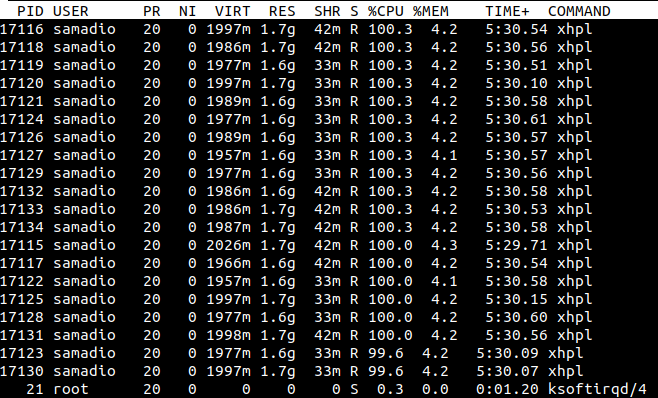
\includegraphics[width=0.7\linewidth]{../usage}
	\caption*{Top output for the HPL benchmark}
	\label{fig:usage}
\end{figure}

The program was run many times in order to get an average, but due to the strcture of the queue system the program has been executed each time in a different node. After comparing the results of the same program, we get the following results.

\begin{figure}[h]
	\centering
	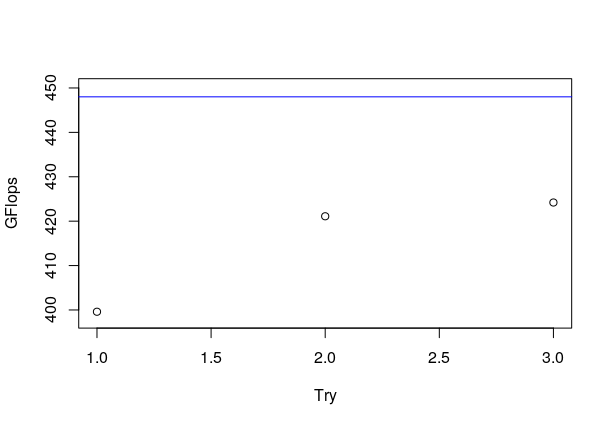
\includegraphics[width=1.\linewidth]{nointel}
	\caption*{Results of HPL benchmark in different nodes}
	\label{fig:nointel}
\end{figure}

The blue line represent the Theoretical Peak Performance(TTP) of a node in the Ulysses cluster, which is 448 GFlops. The graph shows clearly the benchmark achieves more than 90\% of the TTP, with a peak of nearly 95\%.

Despite this excellent results, the oscillations of the values obtained are nearly 5\%, which means that varying a little the input parameter in the file HPL.dat would not give any observable result.

For this reason I decided not to collect any more data

\subsection{Two nodes, 40 processors}

The same process was repeated using two nodes, 40 processors and 40 mpi processes. In this case the values obtained seems to be less dependent on the nodes the program is being executed, so I started modifying the parameter P and Q:
 

\vspace{1mm} % vertical space
\begin{lstlisting}
	
\end{lstlisting}

\section{Appendix: commands and code}

\subsection{HPL library}

In order to download and install the library, I run the following commands:

\vspace{1mm} % vertical space
\begin{lstlisting}
	module load mkl
	module load openmpi/1.8.3/intel/14.0
	wget http://www.netlib.org/benchmark/hpl/hpl-2.2.tar.gz
	tar -xvzf hpl-2.2.tar.gz
	cd hpl-2.2
	cd setup/
	cp Make.Linux_Intel64 ../.
	cd ..
	mv Make.Linux_Intel64 Make.mkl
\end{lstlisting}


Then I proceeded to edit some lines in the Make.mkl file:

\vspace{1mm} % vertical space
\begin{lstlisting}
	ARCH = mkl
	TOPdir = $(HOME)/hpc/ex6/hpl-2.2
	# MPdir        = /opt/intel/mpi/4.1.0
	# MPinc        = -I$(MPdir)/include64
	# MPlib        = $(MPdir)/lib64/libmpi.a
	LAdir        = $(MKLROOT)
\end{lstlisting}

Finally, I run the Makefile in order to create the executable ./xhpl
\vspace{1mm} % vertical space
\begin{lstlisting}
	make arch=mkl
\end{lstlisting}

\subsection{Intel Optimized LINPACK BENCHMARK}
\begin{lstlisting}
	module load mkl
	cd $MKLROOT/ benchmarks/linpack/
	cp /u/shared/programs/x86_64/mkl/11.1.3/composer_xe_2013_sp1.3.174/
		mkl/benchmarks/linpack/xlinpack_xeon64 .
	cp /u/shared/programs/x86_64/mkl/11.1.3/composer_xe_2013_sp1.3.174/
		mkl/benchmarks/linpack/lininput_xeon64 .
\end{lstlisting} 

\subsection{bash script}
\begin{lstlisting}
	## a small script to execute my benchamrk
	
	/bin/hostname #name of the node which is executing my job
	#enter in the right position
	cd hpc/ex6/hpl-2.2/bin/mkl/nthreads
	
	#load modules needed
	module load mkl
	module load openmpi/1.8.3/intel/14.0
	
	#run HPL Benchmark
	
	mpirun -np 20 ./xhpl
	#now the intel
	export OMP_NUM_THREADS=5
	./xlinpack_xeon64 lininput_xeon64
	exit
\end{lstlisting} 
	
\end{document}